\documentclass[a4paper,12pt,titlepage]{ctexart}
\usepackage{graphicx}
\usepackage{multirow}
\usepackage{geometry}
\usepackage{array}
%\author{上海市上海中学\\金佳熠}
\title{\begin{LARGE} \textbf{基于区块链的电子文档交易系统} \end{LARGE}\\[2ex]}
\date{2019年1月}  

\begin{document}         
\maketitle
\thispagestyle{plain}
\setcounter{page}{1}
\pagenumbering{roman}
\tableofcontents
\newpage

\pagestyle{empty}
\noindent \textbf{摘要}:区块链技术,从本质上讲是一种交易记录的存储技术,是基于密码学安全的分布式账簿网络技术.~它对交易记录进行永久性存储,而且存储之后永远无法删除,由此实现对所有的交易历史进行安全的不可篡改的记录.~区块链具有分布式、去中心化、可编程、安全性高、自治性、不可篡改、匿名性等突出特点.~其中去中心化是区块链技术的核心特点,可以基于此解决信任成本的问题,所以区块链技术非常适用于金融、交易等信用交易的场景.~本项目的目标是基于区块链技术搭建一个电子文档交易系统.~不同于传统的中心化交易系统,该系统利用区块链去中心化的特性来实现安全、自治、不可篡改的交易,最终实现电子文档的版权和阅读权的交易功能.~本项目基于以太坊平台,通过智能合约技术来实现核心的交易功能,针对版权和阅读权不同的交易特性,设计了不同的权限校验以及交易逻辑,最终实现了交易系统搭建、交易逻辑设计、交易合约部署以及交易流程验证等核心功能,最后本项目探讨了通过设计特殊专用的电子文档加密和阅读程序,将该程序与区块链的动态权限信息实现实时互通来一定程度上解决电子文档的非法传播和拷贝问题.~\\\par
\noindent \textbf{关键词}:区块链;以太坊;智能合约;去中心化;交易系统;电子文档\\\par
%Abstract: \par
%Key Words: \par
\newpage
\begin{center}
\begin{LARGE}
\textbf{声明}
\end{LARGE}
\end{center}\par
根据《中国人民银行、中央网信办、工业和信息化部、工商总局、银监会、证监会、保监会关于防范代币发行融资风险的公告》文件精神,本项目重点在于探索区块链的应用领域,目前只是进行技术验证,不用于实际运营.~\par
特此声明.~\par
\begin{flushright}
2019年1月
\end{flushright}

\newpage
\setcounter{page}{1}
\pagenumbering{arabic}
\pagestyle{plain}

\section{课题背景}
区块链技术,从本质上讲是一种交易记录的存储技术,是基于密码学安全的分布式账簿网络技术~\cite{pa}.~它对交易记录进行永久性存储,而且存储之后永远无法删除,只能按照次序加入新的交易,由此对所有的交易历史进行永不结束的记载.~区块链具有分布式、去中心化、可编程、安全性高、自治性、不可篡改、匿名性等突出特点.~其中去中心化是区块链技术的核心特点,可以基于此解决信任成本的问题,所以区块链技术非常适用于金融、交易等信用交易的场景.~\par
本文的研究目标是基于区块链技术搭建一个电子文档交易系统,试图解决以下三类问题:\par
1)	电子文档的去中心化存储、质量评价;\par
2)	电子文档版权确权、文档收益归属;\par
3)	扼制电子文档的非法拷贝和侵权传播,保护知识产权.~\par


\section{区块链技术研究现状}
2008年,一位化名为中本聪的人,在一篇为《比特币:一个点对点的电子现金系统》的论文中首先提出了比特币.~中本聪结合以前的多个数字货币发明,如B-money和HashCash,创建了一个完全去中心化的电子现金系统,不依赖于通货保障或是结算验证保障的中央权威.~关键的创新是利用分布式计算系统(称为“工作量证明”算法)每隔10分钟进行一次的全网“选拔”,能够使用去中心化的网络同步交易记录.~比特币打开了区块链的技术大门,区块链技术是比特币原创的核心技术,在比特币被发明之前世界上并不存在区块链这个东西.~ 比特币发明之后,很多人参考比特币中的区块链实现,使用类似的技术实现各种应用,这类技术统称区块链技术.~用区块链技术实现的各种链即为区块链.~
\subsection{区块链原理简介}
区块链的实现方案首先提出一个“时间戳服务器”.~时间戳服务器通过对以区块(block)形式存在的一组数据实施随机散列而加上时间戳,并将该随机散列进行广播,就像在新闻或世界性新闻组网络(Usenet)的发帖一样组成一个楼层链条.~显然,该时间戳能够证实特定数据必然于某特定时刻是的确存在的,因为只有在该时刻存在了才能获取相应的随机散列值.~每个时间戳应当将前一个时间戳纳入其随机散列值中,每一个随后的时间戳都对之前的一个时间戳进行增强, 这样就形成了一个链条.~
\begin{figure}[!hbp]
	\centering
	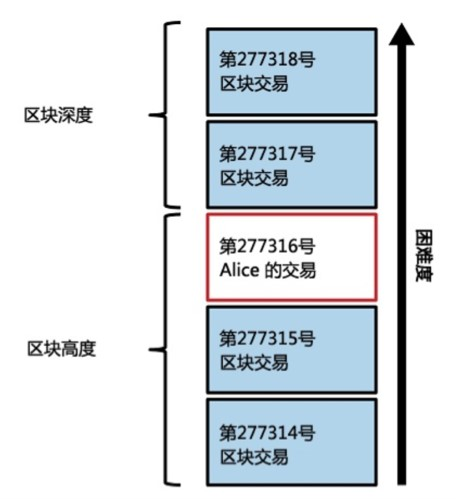
\includegraphics[scale=0.6]{fig1.jpg}
    \caption{区块链形象图}
\end{figure}
\subsection{区块链的共识机制}
区块链解决去中心化的信任问题核心机制是由其独特的共识算法保证的,比较主流的两类共识机制是工作量证明(POW)和权益证明(POS).~\par
比特币采用的共识算法就是POW,区块是在挖矿过程中产生.~所谓挖矿,实际上是穷举随机数算法,把上个区块的哈希值加上10分钟内的全部交易单打包,再加上一个随机数,算出一个256位的字符串哈希值,输入的随机数使哈希值满足一定条件就获得这个区块的交易记账权.~新产生的区块需要快速广播出去,以便其他节点进行对其验证,以防造假.~每个区块存着上一个区块的哈希值,可以溯源到源头,只有经过验证后才最终获得区块的交易记账权.~以比特币的挖矿为例,矿工会根据工作量证明每过特定时间挖到新的区块(如比特币:根据难度系数,工作量证明算法全网算力大概10分钟左右才能产生一个新区块;难度系数会根据全网算力的增加而调整,永远保证大概10分钟产生一个新的区块).~节点会在”父区块哈希值“字段找出包含它的父区块的哈希值.~这是节点已知的哈希值,也就是如下图中第277314块区块的哈希值.~故这个区块是这个链条里的最后一个区块的子区块,因此现有的区块链得以扩展.~节点将新的区块添加到链条的尾端,使区块链变长到一个新的高度277315.~\par
图~\ref{fig2}展示了两个区块的连接:\par
\begin{figure}[!hbp]
	\centering
	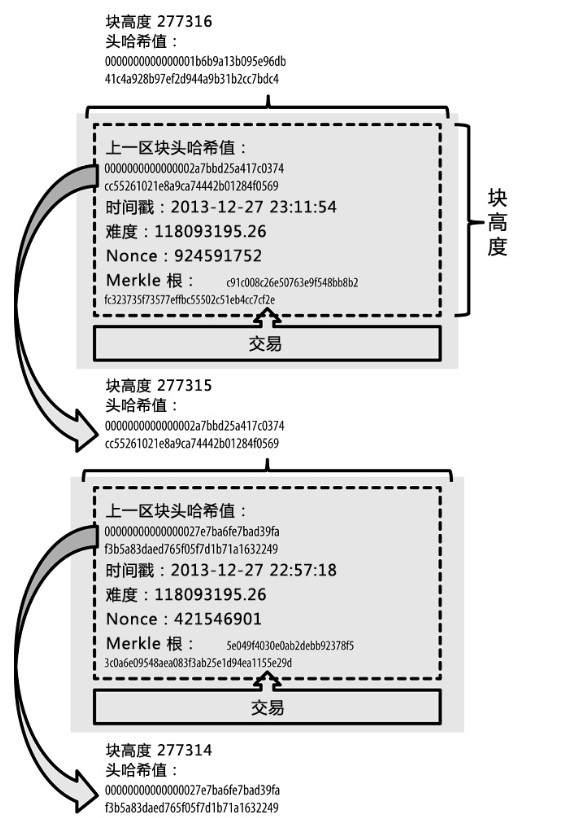
\includegraphics[scale=0.48]{fig2.jpg}
    \caption{区块链接示意图}
    \label{fig2}
\end{figure}
权益证明POS是要求节点提供拥有一定数量的代币证明来获取竞争区块链记账权的一种分布式共识机制.~不同于挖矿机制造成的大量资源浪费以及矿池集中问题,POS机制可以有效降低资源浪费,并缩短共识达成的时间.~


\subsection{比特币创世区块信息}
\begin{figure}[!hbp]
	\centering
	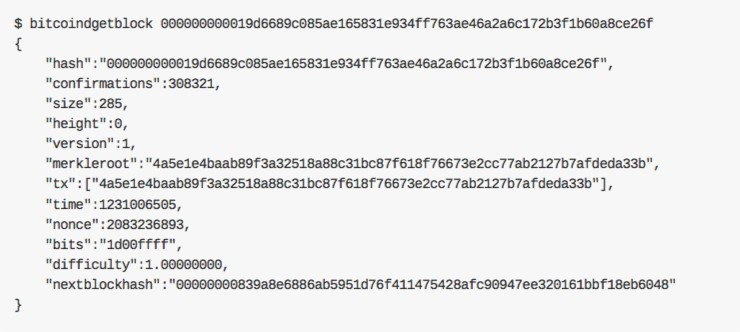
\includegraphics[scale=0.7]{fig3.jpg}
\end{figure}

\subsection{以太坊简介}
「Ethereum(以太坊)」是一个基于区块链的、去中心化的应用平台,它将 比特币的基础设施 —— 基于密码学的区块链技术构建为了一个通用的平台,脚本、竞争币和链上元协议(on-chain meta-protocol)概念进行整合和提高,使得开发者能够创建任意的基于共识的、可扩展的、标准化的、特性完备的、易于开发的和协同的应用.~以太坊通过建立终极的抽象的基础层-内置有图灵完备编程语言的区块链-使得任何人都能够创建合约和去中心化应用,并在其中设立他们自由定义的所有权规则、交易方式和状态转换函数.~\par
在以太坊系统中,状态是由被称为“账户”(每个账户由一个20字节的地址)的对象和在两个账户之间转移价值和信息的状态转换构成的.~以太坊的账户包含四个部分:
\begin{enumerate}
\item 随机数,用于确定每笔交易只能被处理一次的计数器;
\item 账户目前的以太币余额;
\item 账户的合约代码(如果有的话);
\item 账户的存储(默认为空)
\end{enumerate}\par
以太币(Ether)是以太坊内部的主要加密燃料,用于支付交易费用.~一般而言,以太坊有两种类型的账户:外部所有的账户(由私钥控制的)和合约账户(由合约代码控制).~外部所有的账户没有代码,人们可以通过创建和签名一笔交易从一个外部账户发送消息.~每当合约账户收到一条消息,合约内部的代码就会被激活,允许它对内部存储进行读取和写入,和发送其它消息或者创建合约.~其状态转换可以如图~\ref{fig7}描述:\par
\begin{figure}[!hbp]
	\centering
	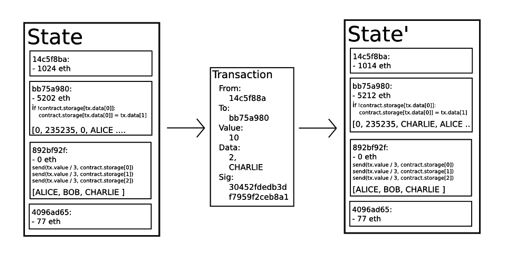
\includegraphics[scale=0.8]{fig7.jpg}
	\caption{以太币的状态转换}
	\label{fig7}
\end{figure}
以太坊的状态转换函数:APPLY(S,TX) $\rightarrow$ S’,可以定义如下:
\begin{enumerate}
\item 检查交易的格式是否正确(即有正确数值)、签名是否有效和随机数是否与发送者账户的随机数匹配;如否,返回错误.~
\item 计算交易费用:~fee=STARTGAS * GASPRICE,并从签名中确定发送者的地址.~从发送者的账户中减去交易费用和增加发送者的随机数.~如果账户余额不足,返回错误.~
\item 设定初值~GAS = STARTGAS,并根据交易中的字节数减去一定量的燃料值.~
\item 从发送者的账户转移价值到接收者账户.~如果接收账户还不存在,创建此账户.~如果接收账户是一个合约,运行合约的代码,直到代码运行结束或者燃料用完.~
\item 如果因为发送者账户没有足够的钱或者代码执行耗尽燃料导致价值转移失败,恢复原来的状态,但是还需要支付交易费用,交易费用加至矿工账户.~
\item 否则,将所有剩余的燃料归还给发送者,消耗掉的燃料作为交易费用发送给矿工.~
\end{enumerate}\par
以太坊合约的代码使用低级的基于堆栈的字节码的语言写成的,被称为“以太坊虚拟机代码”或者“EVM代码”.~代码由一系列字节构成,每一个字节代表一种操作.~一般而言,代码执行是无限循环,程序计数器每增加一(初始值为零)就执行一次操作,直到代码执行完毕或者遇到错误,STOP或者RETURN指令.~操作可以访问三种存储数据的空间:
\begin{enumerate}
\item 堆栈,一种后进先出的数据存储,32字节的数值可以入栈,出栈.~
\item 内存,可无限扩展的字节队列.~
\item 合约的长期存储,一个秘钥/数值的存储,其中秘钥和数值都是32字节大小,与计算结束即重置的堆栈和内存不同,存储内容将长期保持.~
\end{enumerate}\par
代码可以象访问区块头数据一样访问数值,发送者和接受到的消息中的数据,代码还可以返回数据的字节队列作为输出.~\par
以太坊的区块链在很多方面类似于比特币区块链.~它们的区块链架构的不同在于,以太坊区块不仅包含交易记录和最近的状态,还包含区块序号和难度值.~以太坊中的区块确认算法如下:
\begin{enumerate}
\item 检查区块引用的上一个区块是否存在和有效.~
\item 检查区块的时间戳是否比引用的上一个区块大,而且小于15分钟.~
\item 检查区块序号、难度值、 交易根,叔根和燃料限额(许多以太坊特有的底层概念)是否有效.~
\item 检查区块的工作量证明是否有效.~
\item 将S[0]赋值为上一个区块的STATE\_ROOT.~
\item 将TX赋值为区块的交易列表,一共有n笔交易.~对于属于[0,n-1]的i,进行状态转换S[i+1] = APPLY(S[i],TX[i]).~如果任何一个转换发生错误,或者程序执行到此处所花费的燃料(gas)超过了GASLIMIT,返回错误.~
\item 用S[n]给S\_FINAL赋值, 向矿工支付区块奖励.~
\item 检查S\_FINAL是否与STATE\_ROOT相同.~如果相同,区块是有效的.~否则,区块是无效的.~
\end{enumerate}\par
\begin{figure}[!hbp]
	\centering
	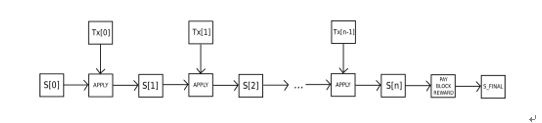
\includegraphics[scale=0.9]{fig8.jpg}
    \caption{以太坊区块确认算法示意图}
\end{figure}
这一确认方法乍看起来似乎效率很低,因为它需要存储每个区块的所有状态,但是事实上以太坊的确认效率可以与比特币相提并论.~原因是状态存储在树结构中(tree structure),每增加一个区块只需要改变树结构的一小部分.~因此,一般而言,两个相邻的区块的树结构的大部分应该是相同的,因此存储一次数据,可以利用指针(即子树哈希)引用两次.~一种被称为“帕特里夏树”(“Patricia Tree”)的树结构可以实现这一点,其中包括了对默克尔树概念的修改,不仅允许改变节点,而且还可以插入和删除节点.~另外,因为所有的状态信息是最后一个区块的一部分,所以没有必要存储全部的区块历史-这一方法如果能够可以应用到比特币系统中,经计算可以对存储空间有10-20倍的节省.~

\newpage
\section{基于区块链的交易}
我们定义,一枚电子货币(an electronic coin)是这样的一串数字签名:每一位所有者通过对前一次交易和下一位拥有者的公钥(Public key) 签署一个随机散列的数字签名,并将这个签名附加在这枚电子货币的末尾,电子货币就发送给了下一位所有者.~而收款人通过对签名进行检验,就能够验证该链条的所有者.~
\subsection{交易流程}
区块链的交易并不是通常意义上的一手交钱一手交货的交易,而是转账.~为了使得价值易于组合与分割,比特币的交易被设计为可以纳入多个输入输出,即一笔交易可以转账给多个人.~一次交易一般分以下几个流程:
\begin{figure}[!hbp]
	\centering
	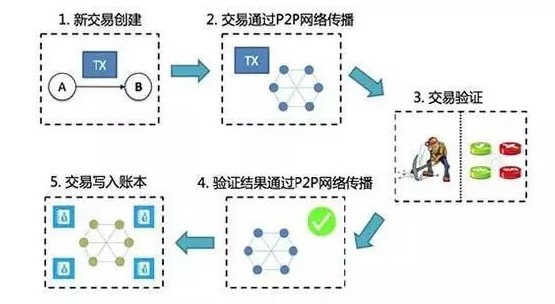
\includegraphics[scale=0.8]{fig4.jpg}
    \caption{区块链交易流程}
\end{figure}
\begin{itemize}
\item 交易的生成\\
当前所有者利用私钥对前一次交易和下一位所有者签署一个数字签名,并将这个签名附加在这枚货币的末尾,制作成交易单.~
\item 交易的传播\\
当前所有者将交易单广播至全网,每个节点都将收到的交易纳入一个区块中.~
\item 共识打成\\
每个节点通过具体的共识算法,竞争获得创建新区块的权力,并争取得到数字货币的奖励.~
\item 整个网络节点的验证\\
当一个节点找到解时,它就向全网广播该区块记录的所有盖时间戳的交易,并由全网其他节点核对.~
\item 记录到区块链\\
全网其他节点核对该区块记账的正确性,没有错误后他们将在该合法区块之后竞争下一个区块,这样就形成了一个合法记账的区块链.~
\end{itemize}

\subsection{交易中的输入与输出}
一笔数字货币的交易是一个含有输入值和输出值的数据结构.~该数据结构植入了将一笔资金从初始点(输入值)转移至目标地址(输出值)的代码信息.~数字货币交易的输入值和输出值与账号或才身份信息无关.~你应该将它们理解成一种被特定密钥信息锁定的一定数量的数字货币.~只有拥有者这个密钥信息的人可以解锁.~\par
一般交易,最常见的交易形式是从一个地址到另一个地址的简单支持.~这种交易也常常包含给支付者”找零“.~\par
集合型交易,是集合多个输入到一个输出的模式,相当于现实生活中将很多硬币和纸币兑换为一个大额面钞.~\par
分散型交易,是将一个输入分配给多个输出,这类交易类似于老板给员工发工资的情形,从一个账号转账给多个账号.~
\subsection{去中心化与安全性保证的技术原理}
为了保证区块的安全性,防止恶意篡改区块信息,同时高效的校验区块信息,以太坊等系统引入了梅克尔帕特里夏树(Merkle Patricia Tree)这种数据结构,简称MPT.~默克尔帕特里夏树由Alan Reiner提出设想,并在瑞波协议中得到实现,是以太坊的主要数据结构,用于存储所有账户状态,以及每个区块中的交易和收据数据.~\par
MPT提供了一个基于加密学的、自校验防篡改的数据结构,用来存储键值对关系(比如每个账户的状态).~MPT具有重要的特性:首先,唯一确定性,确定性是指同样内容的键值,将被保证找到同样的结果,有同样的根哈希,唯一性是指每个数据集仅有一个可能的根散列;其次,高效的更新、添加、或者删除树节点,以及生成新的根散列;第三,无法在不改变根散列的情况下修改树的任何部分,所以如果根散列被包括在签名的文档或有效区块中话,签名或工作证明可以担保整个树不被篡改;第四,任何人只可以提供一个下到特定节点的分支,可以以加密的方式高效地证明拥有确切内容的节点确实包含在树里.~\par
关于效率方面,对树的插入,查找,删除的时间复杂度控制在O(log(n)).~相较于红黑树来说,MPT更好理解和编码实现.~

\newpage
\section{基于区块链的文档交易系统}
本研究课题提出基于区块链技术来实现一套电子文档交易系统.~类似比特币的第一代区块链技术只能实现简单的去中心化的不可篡改的分布式权益登记,然而新时代的交易系统往往需要在交易时增加附加条款功能,以满足在不同条件达成时触发不同的交易权益,这里最典型的就是保险交易,用户购买保险后,最终是否发生理赔,以及理赔的额度是由未来某个时刻具体情况所决定的,不可篡改的固定式的权益登记显然不能满足此类需求.~为了解决此类问题智能合约应运而生.~一个智能合约是一套以数字形式定义的承诺,包括合约参与方可以在上面执行这些承诺的协议.~智能合约可以实现严格按照交易双方约定的规则来实现交易以及交易中约定的在未来执行的附属条款.~\par
本交易系统是基于智能合约的区块链交易系统,除了区块链本身的去中心化、安全性高、匿名性等特点外,还能够通过智能合约支持各种多样化的交易需求.~为了实现带有智能合约的交易系统,从零开始实现显然是不现实的,为此我们参考区块链2.0的技术架构(其基本架构如下图所示),基于以太坊平台来进行扩展.~本研究课题的目标便是借鉴区块链2.0的技术方案来实现一套可用的去中心化的交易系统.~\par
\begin{figure}[!hbp]
	\centering
	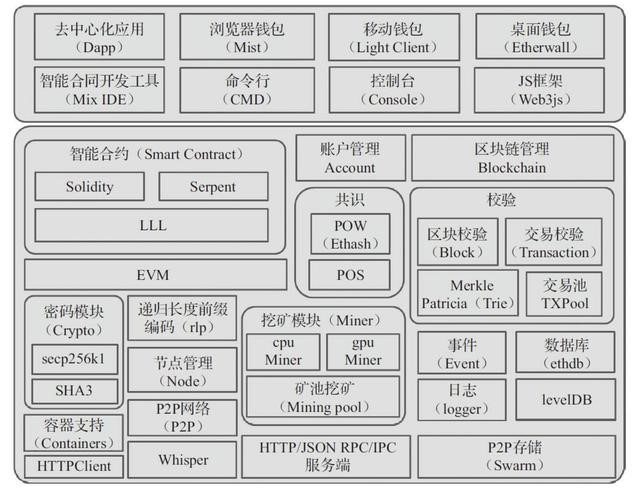
\includegraphics[scale=0.6]{fig6.jpg}
	\caption{以太坊架构}
\end{figure}
\subsection{智能合约}
一个智能合约是一套以数字形式定义的承诺,包括合约参与方可以在上面执行这些承诺的协议.~一个合约由一组代码(可以理解为合约的函数)和数据(即合约的状态)组成,并且运行在以太坊虚拟机上.~智能合约的代码,可以读取交易数据,在自己的存储空间写入数据,读取区块状态数据,向另一个合约发送一个内部交易,这个功能的组合可以满足多样化的交易需求.~\par
以太坊虚拟机(EVM)是以太坊智能合约的运行环境,他被沙箱封装起来,与网络、文件系统或其他进程完全隔离,创造了一个安全干净的运行环境.~以太坊虚拟机使用了256比特长度的机器码,是一种基于堆栈的虚拟机,用于执行以太坊智能合约 .~由于EVM是针对以太坊体系设计的,因此使用了以太坊账户模型(Account Model)进行价值传输.~以太坊中有两类账户,它们共用同一个地址空间.~一类是外部账户,该类账户被公钥-私钥对控制(人类).~另一类是合约账户,该类账户被存储在账户中的代码控制.~\par
外部账户的地址是由公钥决定的,合约账户的地址是在创建该合约时确定的(这个地址由合约创建者的地址和该地址发生过的交易计算得到,地址发出过的交易数量也被称作"nonce")\par
合约账户存储了代码,外部账户则没有,除了这点以外,这两类账户对于EVM来说是一样的.~每个账户有一个key-value形式的持久化存储.~其中key和value的长度都是256bit,名字叫做storage.~另外,每个账户都有一个以太币余额(单位是“Wei"),该账户余额可以通过向它发送带有以太币的交易来改变.~
\subsection{账户交易}
一笔交易实际上是一条消息,从一个账户发送到另一个账户(也可能是相同的账户或者零账户).~交易可以包含二进制数据(payload)和以太币.~如果目标账户包含代码,该代码会执行,payload就是输入数据.~如果目标账户是零账户(账户地址是0),交易将创建一个新合约.~正如上文所讲,这个合约地址不是零地址,而是由合约创建者的地址和该地址发出过的交易数量(被称为nonce)计算得到.~以太坊上的每笔交易都会被收取一定数量的gas,gas的目的是限制执行交易所需的工作量,同时为执行支付费用.~当EVM执行交易时,gas将按照特定规则被逐渐消耗.~gas价格是由交易创建者设置的,如果执行结束还有gas剩余,这些gas将被返还给发送账户.~无论执行到什么位置,一旦gas被耗尽,将会触发一个gas耗尽异常.~当前调用帧所做的所有状态修改都将被回滚.~\par
\begin{figure}[!hbp]
	\centering
	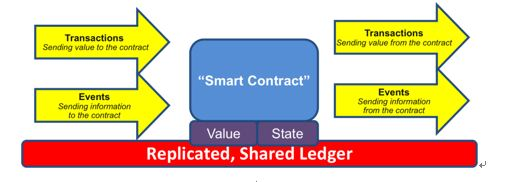
\includegraphics[scale=0.9]{fig9.jpg}
	\caption{基于智能合约的交易示意图}
\end{figure}
本文的交易系统的交易流程如下图所示,交易双方根据具体情况商定合同细节,将合同转换为合约逻辑,并用脚本语言实现,接着编译合约并将合约提交到区块链网络上,所有节点验证成功后接受此合约,代表合约部署成功,至此合约开始执行且不可更改.~\par
\begin{figure}[!hbp]
	\centering
	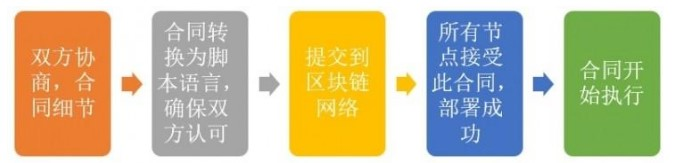
\includegraphics[scale=0.6]{fig5.jpg}
	\caption{交易流程}
\end{figure}
这里用于实现合约的脚本语言是Solidity,是一种智能合约高级语言,可以运行在EVM之上,其语法接近于Javascript,是一种面向对象的语言.~Solidity 是静态类型语言,支持继承、库和复杂的用户定义类型等特性.~除了具备基本程序语言的特性外,还具有以下特点:
\begin{enumerate}
\item 异常机制,类似于事务的原子性.~一旦出现异常,所有的执行都将会被回撤,这主要是为了保证合约执行的原子性,以避免中间状态出现的数据不一致.~
\item 运行环境是在去中心化的网络上,会比较强调合约或函数执行的调用的方式.~因为原来一个简单的函数调用变为了一个网络上的节点中的代码执行
\item 存储是使用网络上的区块链,数据的每一个状态都可以永久存储.~
\end{enumerate}\par
\subsection{交易系统智能合约设计}
一个最简单的合约架构可以表示为数据合约和逻辑合约两层架构,如下图所示.~这样分层的原因是为了方便后期合约的升级.~\par
\begin{figure}[!hbp]
	\centering
	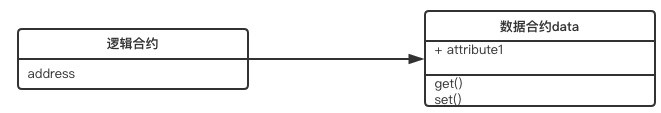
\includegraphics[scale=0.6]{fig10.jpg}
	\caption{简单的智能合约结构}
\end{figure}
一个交易的智能合约,需要包含交易基本上下文,包括交易标的、交易时间、交易出售者地址、交易购买者地址、当前交易状态、交易发生的条件,此外还需要约定交易条件,包括交易达成的条件,交易价格,交易终止的条件等.~将上述交易数据和交易逻辑,打包实现成智能合约的形式,部署到区块链上,并作为一个模板开发给第三方使用,即可形成一个交易系统.~\par
具体的工作包括以太坊区块链平台的搭建和部署,solidity开发环境的配置和调试,solidity合约语言特性的学习,合约的实现、测试和部署.~附录A基于solidity实现了一个交易合约的demo.~\par

\subsection{交易系统设计}
线上交易系统是一个包括交易前端、交易服务器、存储服务器以及其他辅助系统组成的一套复杂系统,一般包括交易数据、交易规则、交易校验、风险控制、仓储控制等系统,线上交易系统是指设计一套软件来组织上述模块.~\par
\begin{figure}[!hbp]
	\centering
	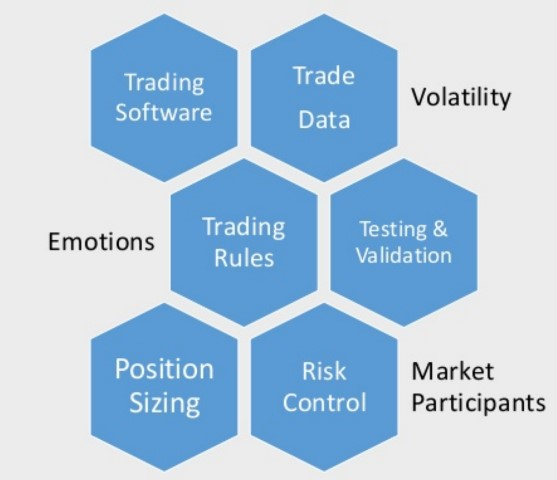
\includegraphics[scale=1.3]{fig11.jpg}
	\caption{交易系统架构}
\end{figure}
一个中心化的简化交易系统一般包括客户端、服务器两部分.~客户端承载了商家的商品发布、消费者商品浏览、下订单、发起支付、商家与消费者的交流展示等功能;服务器负责所有的数据存储、逻辑运行、商品更新推荐、交易处理、异常检测与恢复等核心功能.~下图给出了一个商用的交易系统的包含的各类模块.~\par
\begin{figure}[!hbp]
	\centering
	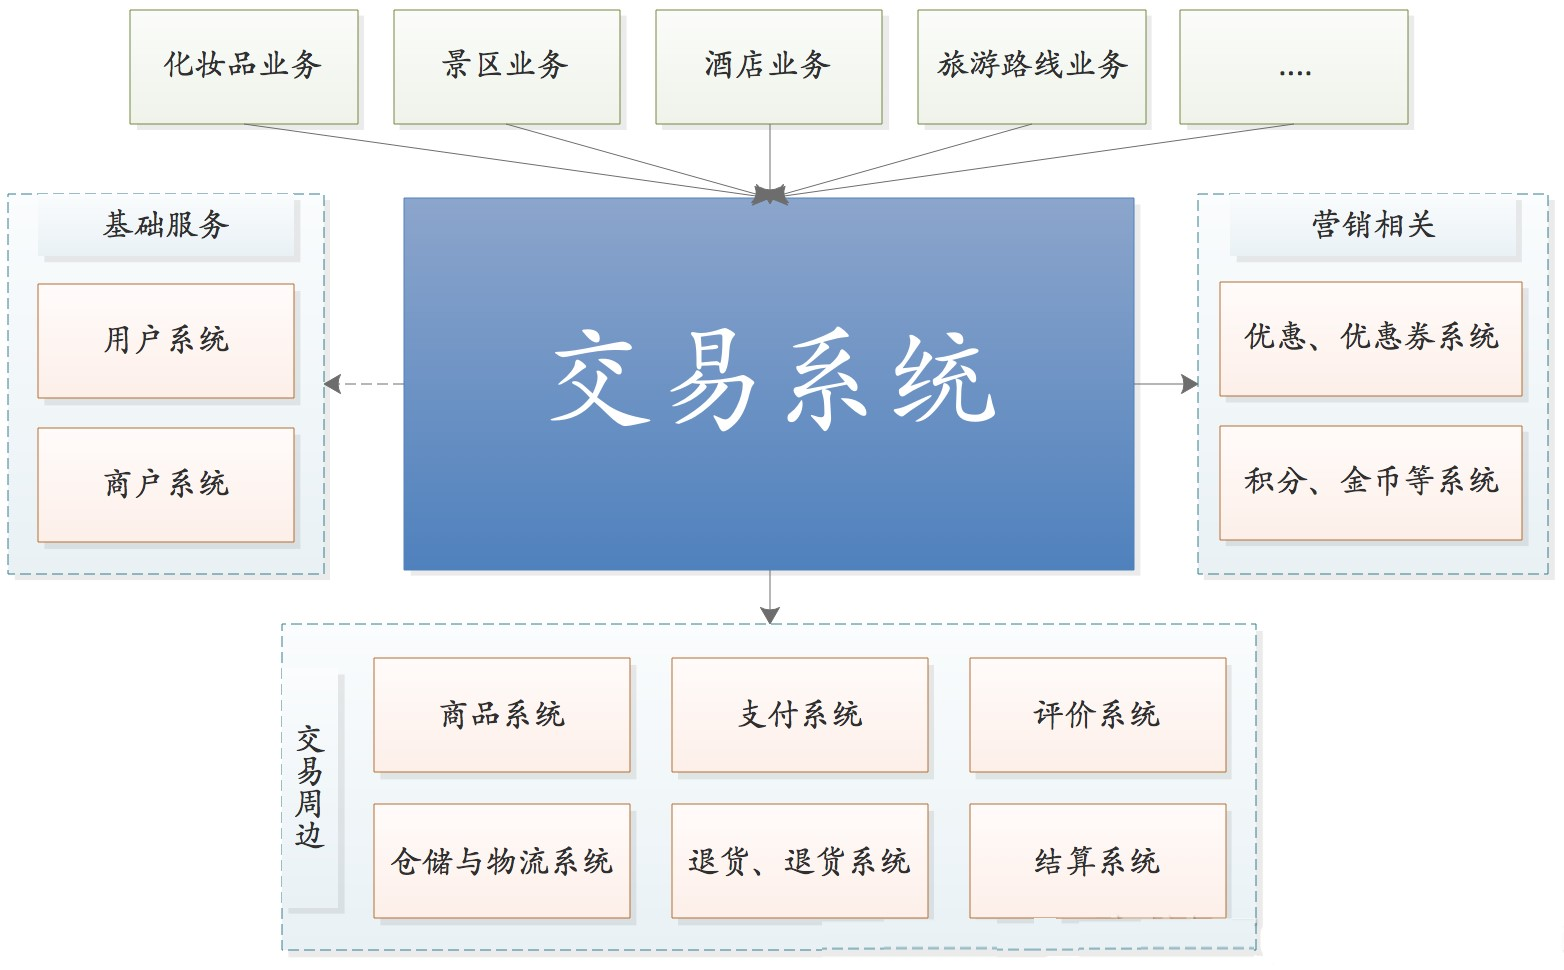
\includegraphics[scale=0.3]{fig12.jpg}
	\caption{交易系统组成}
\end{figure}
不同于中心化的交易系统,基于区块链的交易系统最核心的特质便是去中心化,这时候就需要摈弃或者部分摈弃中心化的客户端-服务器模式,把最核心的交易逻辑和交易数据上链,实现去中心化的交易.~图~\ref{fig13}~给出一个基于以太坊的交易系统的基本结构.~\par
\begin{figure}[!hbp]
	\centering
	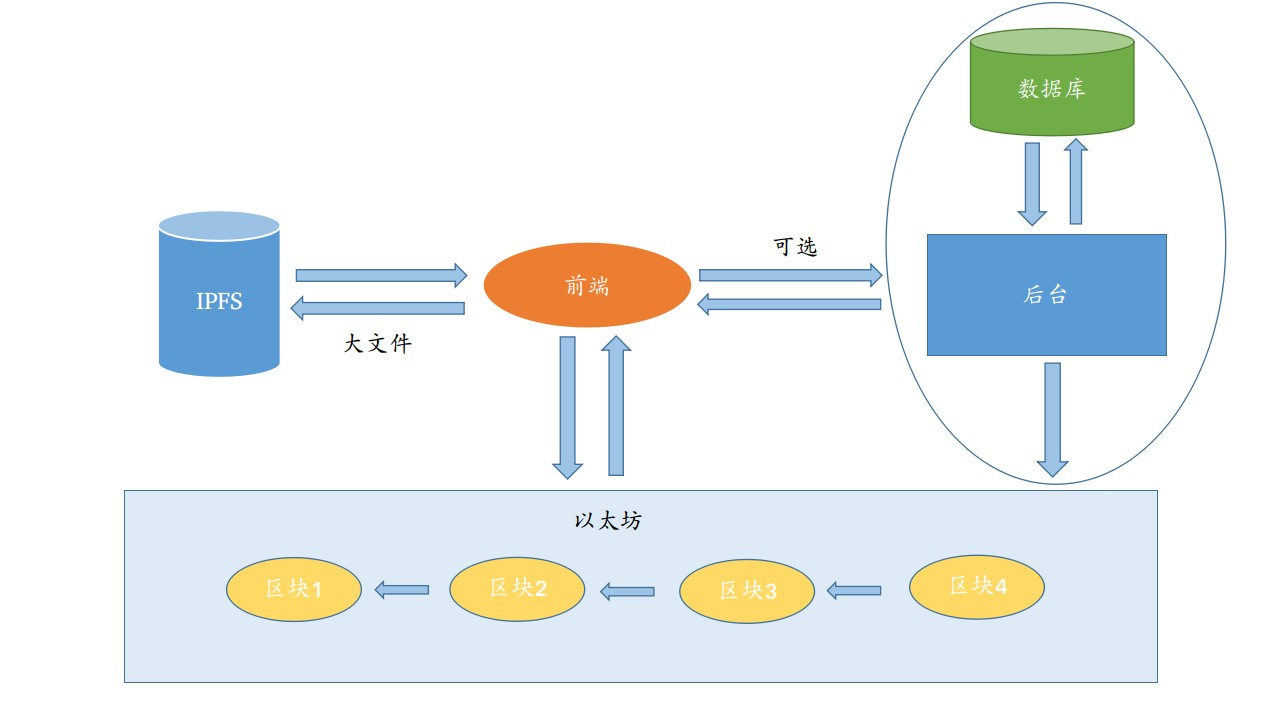
\includegraphics[scale=0.30]{fig13.jpg}
	\caption{交易系统结构}
	\label{fig13}
\end{figure}
对于电子书的交易而言,其实包含了两类不同的交易,一类是版权的交易,一类是阅读权的交易.~对于前者而言,交易之前出售者拥有电子书的版权,交易双方商定具体的交易细节(以智能合约的形式呈现),发生交易后,出售者将电子书的版权让渡给购买者来获得一定的收益,购买者以一定的代价拿到了电子书的版权,同时将交易状态上链,区块链对交易合法性以及版权的所有方进行认证,由于区块链特有的去中心化和防篡改的特性,非常适合实现此类交易.~对于阅读权的交易而言,限定只有拥有电子书版权的账户才具有此类交易权限,可以将阅读权按照一定的约定交易给购买者,购买者获得阅读权之后,有权阅读该文档,当无权在系统里交易文档,这个特性同样需要区块链的权限认证来进行保护和限制,这些可以借助账户签名技术和非对称加密技术来实现.~为实现上述特性,我们提出的整体的系统架构如图~\ref{fig14}~所示:\par
\begin{figure}[!hbp]
	\centering
	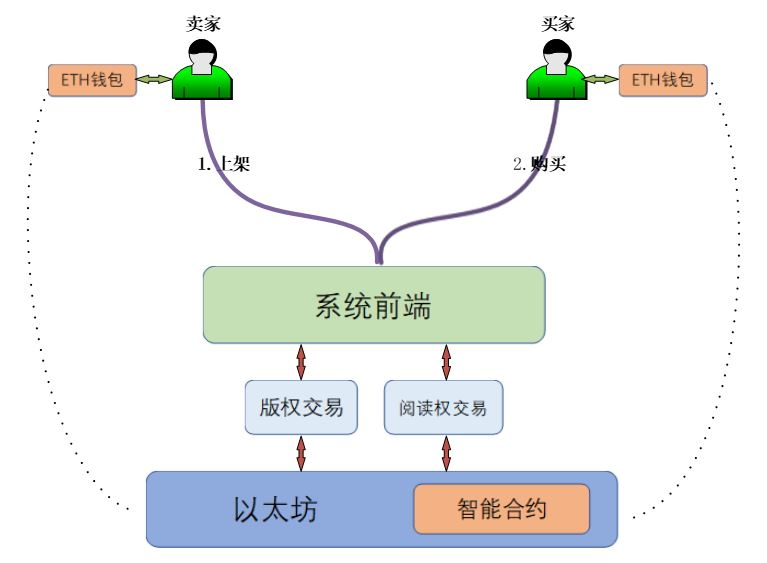
\includegraphics[scale=0.5]{fig14.jpg}
	\caption{电子文档交易系统架构}
	\label{fig14}
\end{figure}
对于阅读权交易而言,首先只有拥有版权的一方才可以出售阅读权,其他人只能购买阅读权,所以权限核查是首先要进行,不满足权限的交易行为是会被立即禁止的.~交易上架后,如果有购买者发起购买交易,接着会进入智能合约逻辑,合约针对钱包地址,双方权限,双方所有物以及双方的财产进行校验,校验成功后发起交易转账,并扣除交易成本,接着对文档进行加密传输给购买者,并赋予购买者阅读权限以及加密的文档.~后面可以进行阅读,但不能出售.~获得阅读权的买家,每次阅读时,都会走校验流程,查看文档是否是正版文档(这个一般需要在加密文档时,将文档的版权所有者地址以及对应的签名一起打包进入文档数据中,以方便后序校验),同时校验玩家是否有阅读权限,校验通过后,可利用解密程序对文档复原,以供阅读.~\par
阅读权的交易流程如图~\ref{fig17}~所示,阅读流程如图~\ref{fig18}~所示.~\par
\begin{figure}[!hbp]
	\centering
	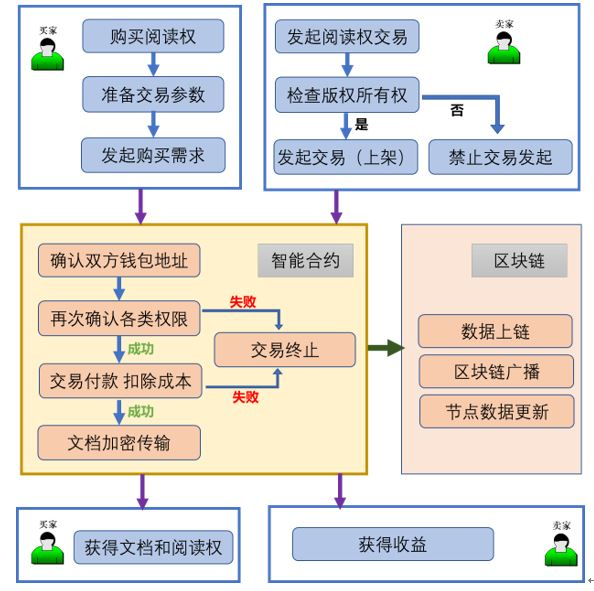
\includegraphics[scale=0.6]{fig17.jpg}
	\caption{阅读权的交易流程}
	\label{fig17}
\end{figure}
\begin{figure}[!hbp]
	\centering
	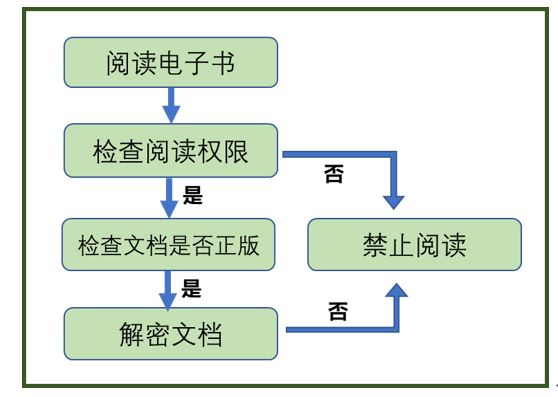
\includegraphics[scale=0.5]{fig18.jpg}
	\caption{阅读流程}
	\label{fig18}
\end{figure}
对于版权交易而言,显然拥有版权的一方才可以出售阅读权,其他人只能购买.~与阅读权交易一样权限核查是首先要进行,不满足权限的交易行为会被立即禁止的.~版权交易上架后,如果有购买者发起购买交易,接着会进入智能合约逻辑,合约针对钱包地址,双方权限,双方所有物以及双方的财产进行校验,校验成功后发起交易转账,并扣除交易成本,接着对版权权限进行更新,出售方失去版权获得收益,购买方获得版权,这些数据通过区块链进行全局广播,所有节点更新对应信息.~同时对文档进行加密传输给购买者,出售者的版权权限和阅读权权限同时失效.~获得版权的买家,以后可以交易阅读权和版权.~具体流程如图~\ref{fig20}~所示.~\par
\begin{figure}[!hbp]
	\centering
	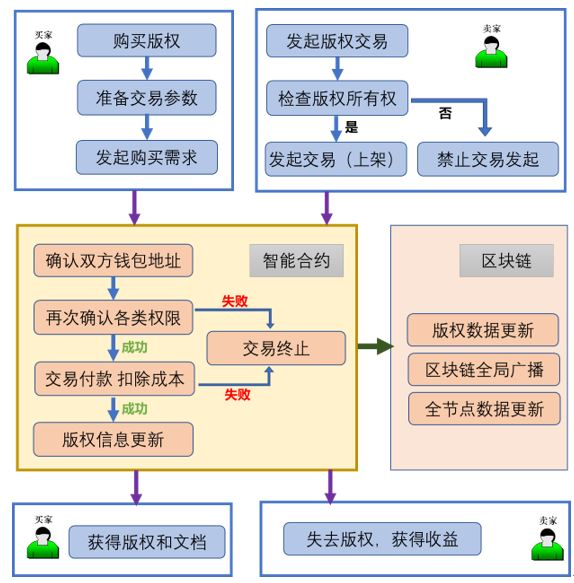
\includegraphics[scale=0.5]{fig20.jpg}
	\caption{版权交易流程}
	\label{fig20}
\end{figure}

\newpage
\section{文件存储和权限校验问题}
区块链去中心化的性质决定了随着越来越多区块的加入,区块链的信息量只会一直增大.~虽然扩容可以解决区块容量过小而造成交易拥堵情况严重的问题,但扩容并没有办法减少信息总量.~本项目的电子文档数据如果全部上链,必然会随着交易量提升导致链上数据过于庞大,这对本地节点的同步以及全链共识的行程都会有效率上的影响.~为了解决这个问题,我们提出引入星际文件系统(IPFS, Inter Planetary File System)存储模式来解决.~IPFS是一个旨在创建持久且分布式存储和共享文件的网络传输协议,是一种内容寻址的对等超媒体分发协议.~在IPFS网络中的节点构成一个分布式文件系统.~\par
在2014年,IPFS协议利用比特币区块链协议和网络基础设施的优势来存储不可更改的数据,移除网络上的重复文件,以及获取存储节点的地址信息——用以搜索网络中的文件.~IPFS是通用目的的基础架构,基本没有存储上的限制.~大文件会被切分成小的分块,下载的时候可以从多个服务器同时获取,可以很好的适应内容分发网络(CDN)的要求.~IPFS文件还可以抽象成特殊的IPFS目录,从而标注一个可读的文件名(透明的映射到IPFS哈希),在访问的时候会像HTTP一样获取一个目录索引.~由于IPFS/IPNS的哈希值都是很长和难记的字符串,所以IPFS兼容了现存的域名系统(DNS),可以通过可读的链接访问IPFS/IPNS内容.~\par
\begin{figure}[!hbp]
	\centering
	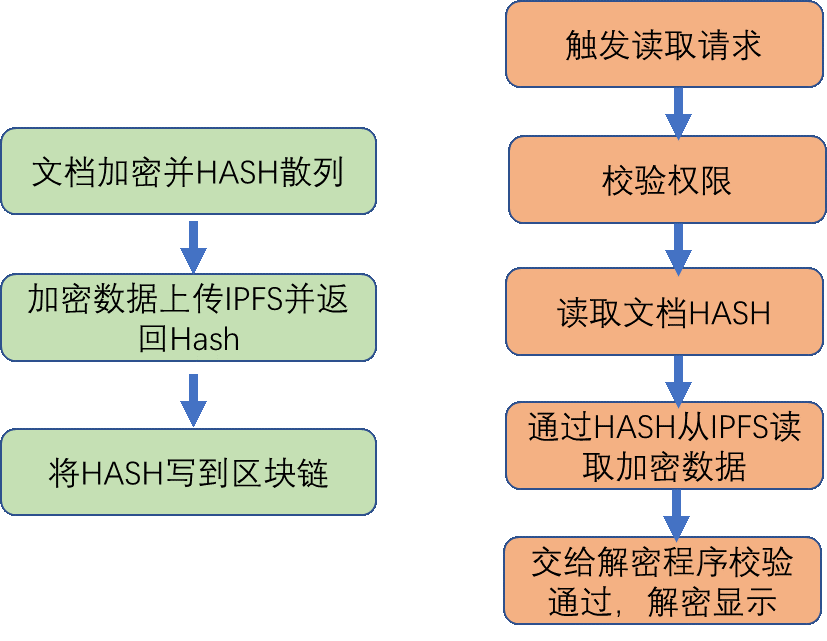
\includegraphics[scale=0.5]{fig23.png}
	\caption{基于IPFS的文档数据存储和读取流程}
\end{figure}
本项目将实体的电子文档数据分离处理出来单独存储到IPFS服务器上,区块链中只存储文档的哈希以及各种权限和交易信息.~这样整体的项目架构变更为如下结构,分为链上链下两级结构,这样可以很好的解决数据同步和效率瓶颈问题.~\par
对于获得阅读权的玩家而言,需要经过权限的验证以及通过专门的解密程序方可打开并阅读电子文档.~区块链本身是可以传输并保存数据的,但是文档数据一般较大,放在区块链上直接传输不够经济有效,所以本项目我们设计区块链只记录交易状态和权限、签名等信息,文档数据放在非中心化的数据库中,独立于区块链存储,同时对文档进行特殊的加密,并设计开发专门的应用程序进行校验后方可解密查看,该应用会和区块链中存贮的权限和签名信息进行动态通信,用来实时校验文档的权限有效性.~通过此方案可以解决电子文档的存储,并从某种程度上杜绝文档的非法拷贝.~

\newpage
\section{项目实践}
\subsection{合约交易逻辑时间}
本项目基于以太坊平台开发,交互前端用了Ethereum Wallet\footnote{\mbox{https://github.com/ethereum/mist/releases}}.~Ethereum Wallet性能稳定高效,同步速度快,且内置了共识引擎,方便基于图形客户端进行合约的开发、调试测试.~进入官方下载对应的前端安装文件,开始安装.~安装好后运行程序,就可以建立钱包,输入账户名、密码即可建立钱包,同时获得了唯一的用户地址,该地址是所有交易校验权限的核心.~\par
开发框架基于Truffle,依赖于Node.js.~开发环境需要配置Node, 使用npm安装所需的依赖包,包括Truffle开发框架,Mocha部署框架等.~然后通过Solidity语言开发好智能合约后,就可以基于上述开发环境进行编译、测试和部署.~\par
本项目使用以太坊节点的Go语言实现版本Geth为基本的实践平台,交互前端用了Ethereum Wallet钱包,此外使用Remix作为合约DApp的集成开发环境,完成合约代码的开发测试和部署.~\par
开发之前首先需要搭建以太坊私链环境,便于环境测试和部署.~首先安装Geth环境.~\par
\begin{figure}[!hbp]
	\centering
	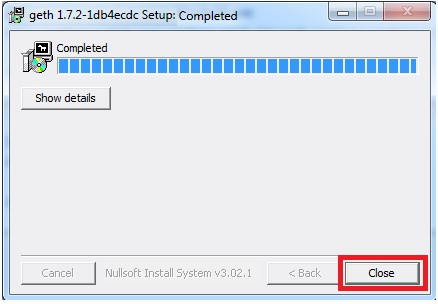
\includegraphics[scale=0.80]{fig21.jpg}
	\caption{Geth安装界面}
\end{figure}
利用Geth首先生成创世区块,并初始化以太坊私链网络.~\par
\newpage
\begin{figure}[!hbp]
	\centering
	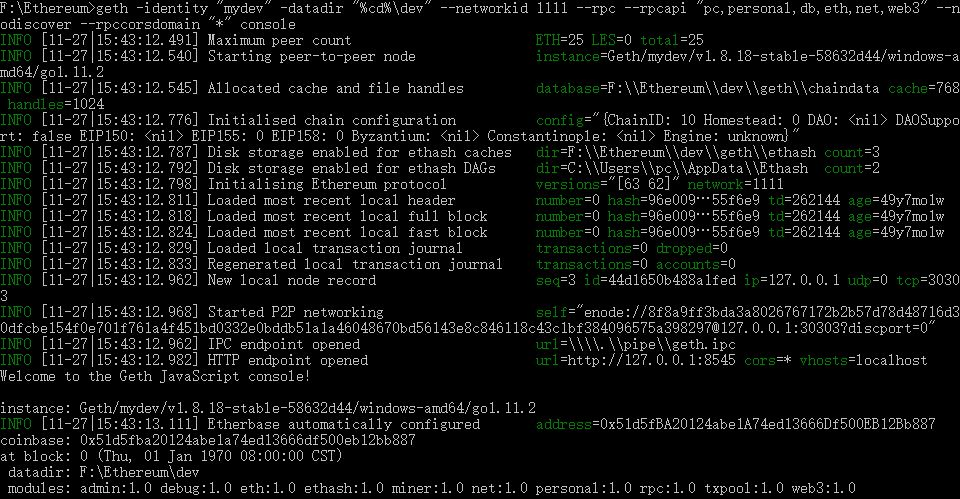
\includegraphics[scale=0.5]{fig19.jpg}
	\caption{私有链启动}
\end{figure}
将Ethereum Wallet客户端连接到私链上,就可以查看并操作对应的账户.~这样开发和运行环境就基本就绪了.~接着可以通过Remix来开发DApp应用,进而进行测试和部署.~
\begin{figure}[!hbp]
	\centering
	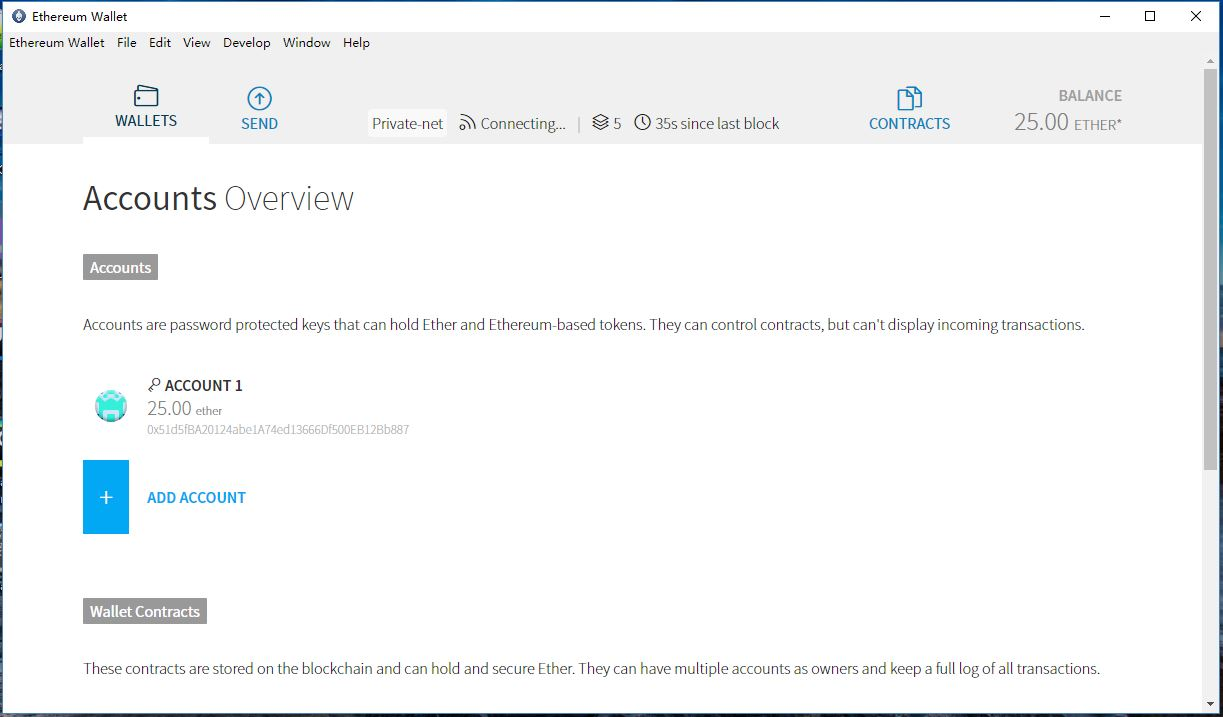
\includegraphics[scale=0.36]{fig15.jpg}
	\caption{Ethereum Wallet交互界面}
\end{figure}
\begin{figure}[!hbp]
	\centering
	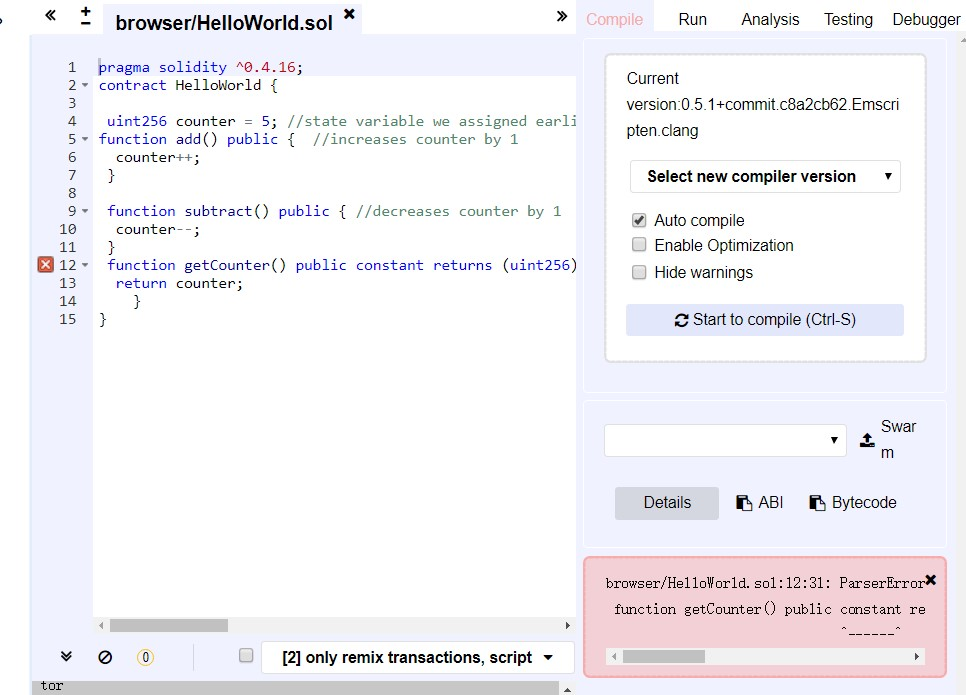
\includegraphics[scale=0.50]{fig22.jpg}
	\caption{Remix IDE界面}
\end{figure}
%\begin{figure}[!hbp]
%	\centering
%	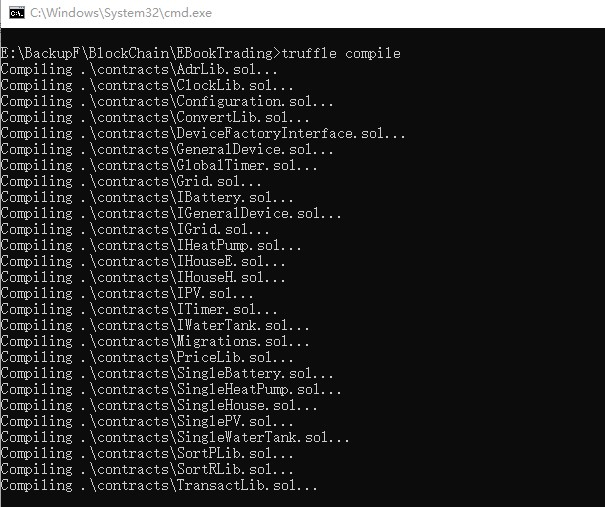
\includegraphics[scale=0.5]{fig16.jpg}
%	\caption{合约编译}
%\end{figure}
\newpage
\subsection{IPFS实践}
首先进行IPFS环境配置,安装IPFS本地环境.~然后创建IPFS节点,根据需要还可以修改节点的默认存储空间.~配置后就可以启动节点服务器了.~\par
\begin{verbatim}
localhost:.ipfs admin$ ipfs daemon
Initializing daemon...
Adjusting current ulimit to 2048...
Successfully raised file descriptor limit to 2048.
Swarm listening on /ip4/111.196.241.208/tcp/7723
Swarm listening on /ip4/127.0.0.1/tcp/4001
Swarm listening on /ip4/192.168.0.107/tcp/4001
Swarm listening on /ip6/::1/tcp/4001
API server listening on /ip4/127.0.0.1/tcp/5001
Gateway (readonly) server listening on /ip4/127.0.0.1/tcp/8080
Daemon is ready
\end{verbatim}\par
接下来我们可以创建react app工程来实现ipfs数据的上传和下载,下面简单介绍一个小示例.~
\begin{enumerate}
\item 安装create-react-app
	\begin{verbatim}
	localhost:1123 admin$ npm install -g create-react-app
	\end{verbatim}

\item React项目创建
	\begin{verbatim}
	localhost:1123 admin$ create-react-app ipfs-http-demo
localhost:ipfs-http-demo admin$ ls
README.md	package.json	src
node_modules	public		yarn.lock
localhost:ipfs-http-demo admin$
	\end{verbatim}

\item 运行React项目
	\begin{verbatim}
	localhost:ipfs-http-demo admin$ npm start
Compiled successfully!

You can now view ipfs-http-demo in the browser.

  Local:            http://localhost:3000/
  On Your Network:  http://192.168.0.107:3000/

Note that the development build is not optimized.
To create a production build, use yarn build.

	\end{verbatim}
	
\item 安装ipfs-api
	\begin{verbatim}
	npm uninstall --save ipfs-api
	\end{verbatim}
	
\item 完成UI逻辑(附部分前端代码)
\begin{footnotesize}


	\begin{verbatim}
	import React, {Component} from 'react';
import './App.css';

const ipfsAPI = require('ipfs-api');
const ipfs = ipfsAPI({host: 'localhost', port: '5001', protocol: 'http'});

class App extends Component {

  constructor(props) {
    super(props);
    this.state = {
      strHash: null,
      strContent: null
    }
  }

  saveTextBlobOnIpfs = (blob) => {
    return new Promise(function(resolve, reject) {
      const descBuffer = Buffer.from(blob, 'utf-8');
      ipfs.add(descBuffer).then((response) => {
        console.log(response)
        resolve(response[0].hash);
      }).catch((err) => {
        console.error(err)
        reject(err);
      })
    })
  }

  render() {
    return (<div className="App">
      <input ref="ipfsContent" style=/>
      <button onClick={() => {
          let ipfsContent = this.refs.ipfsContent.value;
          console.log(ipfsContent);
          this.saveTextBlobOnIpfs(ipfsContent).then((hash) => {
            console.log(hash);
            this.setState({strHash: hash});
          });
        }}>提交到IPFS</button>

      <p>{this.state.strHash}</p>

      <button onClick={() => {
          console.log('从ipfs读取数据')
        }}>读取数据</button>
      <h1>{this.state.strContent}</h1>
    </div>);
  }
}

export default App;
	\end{verbatim}
\end{footnotesize}
\end{enumerate}

以上传图片类型的文件为例,最终实现效果为:
\begin{figure}[!hbp]
	\centering
	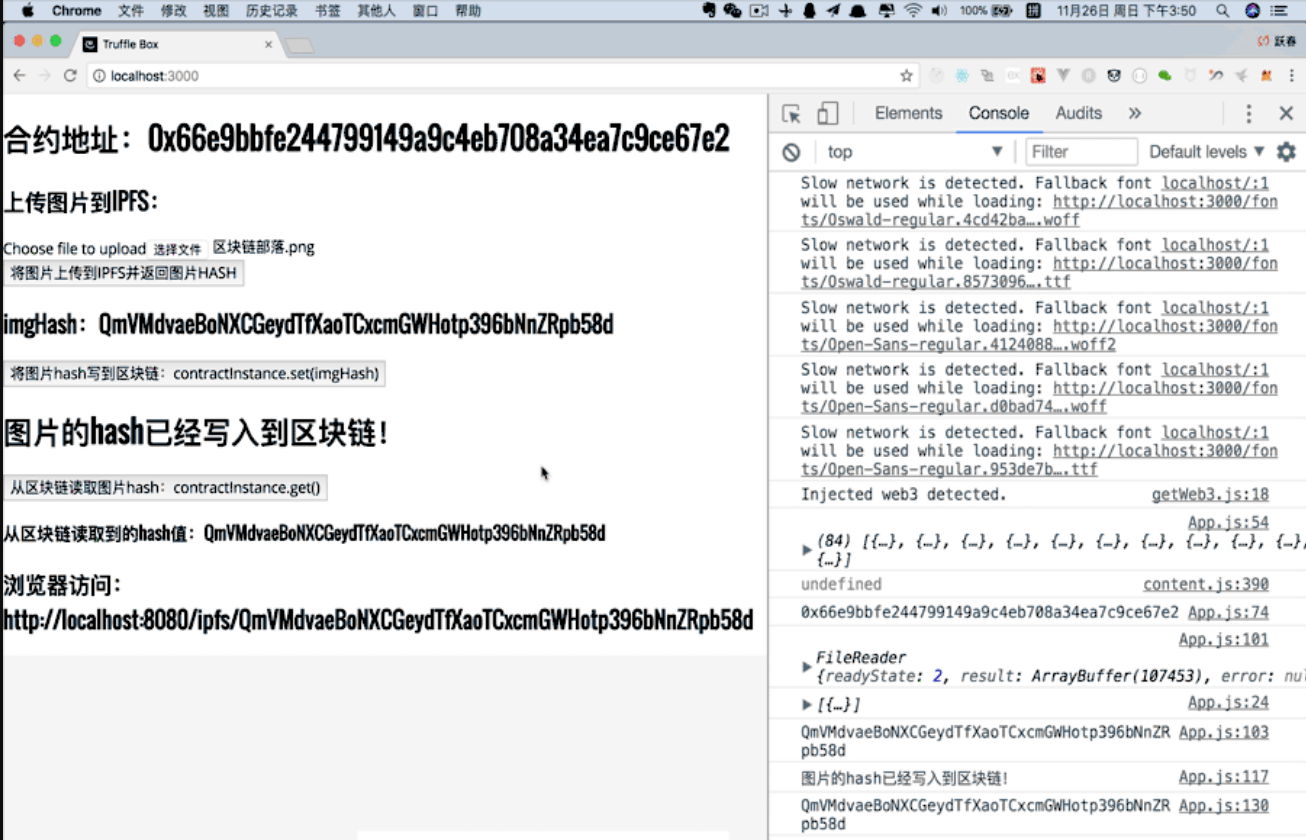
\includegraphics[scale=0.36]{fig24.png}
	\caption{上传图片类型文件的实现效果}
\end{figure}

\newpage
\section{总结与展望}
本项目基于以太坊平台,通过智能合约技术来实现核心的交易功能,针对版权和阅读权不同的交易特性,设计了不同的权限校验以及交易逻辑,最终实现了交易系统搭建、交易逻辑设计、交易合约部署以及交易流程验证等核心功能,另外针对区块链对于容量数据的同步问题引发的效率问题,我们提出通过引入IPFS分布式存储服务器来解决此问题,从而很好地解决了数据存储同步以及链上的存储瓶颈问题.~\par
最后需要关注的一个问题是电子文档数据容易引发非法拷贝问题,对于获取了阅读权限的用户而言,如果将电子文档通过当前主流的阅读器来提供阅读服务,那么此类非法拷贝问题想必会很容易发生,这会对我们的交易系统生态造成非常大的影响.~为了解决此问题,在此我们提出通过设计特殊专用的电子文档加密和阅读程序,将该程序与区块链的动态权限信息实现实时互通,并通过特殊的加密机制来加密存储在IPFS服务器上的文档数据,数据从服务器上下载之前首先需要到区块链校验权限信息,并获取文档散列标签以及匹配解密的秘钥信息,然后通过我们特殊的应用程序来实现解密数据,最终才能提供阅读服务.~这样就算玩家通过非正常途径获取了数据,也不能正常阅读,从而一定程度上解决电子文档的非常传播和拷贝问题.~这部分工作已经开始进行,并会在后续逐步完善.~

\newpage
\newgeometry{left = 1.5 cm, right = 1.5 cm}
\section{附录}
\subsection*{附录A 基于Solidity的交易合约demo代码}
\begin{scriptsize}
\begin{verbatim}
// B3log Token
//   https://hacpai.com
//   https://github.com/b3log
pragma solidity ^0.4.18;

/**
 * @title SafeMath
 * @dev Math operations with safety checks that throw on error
 */
library SafeMath {

  /**
  * @dev Multiplies two numbers, throws on overflow.
  */
  function mul(uint256 a, uint256 b) internal pure returns (uint256) {
    if (a == 0) {
      return 0;
    }
    uint256 c = a * b;
    assert(c / a == b);
    return c;
  }

  /**
  * @dev Integer division of two numbers, truncating the quotient.
  */
  function div(uint256 a, uint256 b) internal pure returns (uint256) {
    // assert(b > 0); // Solidity automatically throws when dividing by 0
    uint256 c = a / b;
    // assert(a == b * c + a % b); // There is no case in which this doesn't hold
    return c;
  }

  /**
  * @dev Substracts two numbers, throws on overflow (i.e. if subtrahend is greater than minuend).
  */
  function sub(uint256 a, uint256 b) internal pure returns (uint256) {
    assert(b <= a);
    return a - b;
  }

  /**
  * @dev Adds two numbers, throws on overflow.
  */
  function add(uint256 a, uint256 b) internal pure returns (uint256) {
    uint256 c = a + b;
    assert(c >= a);
    return c;
  }
}

/**
 * @title Ownable
 * @dev The Ownable contract has an owner address, and provides basic authorization control
 * functions, this simplifies the implementation of "user permissions".
 */
contract Ownable {
  address public owner;

  event OwnershipTransferred(address indexed previousOwner, address indexed newOwner);

  /**
   * @dev The Ownable constructor sets the original `owner` of the contract to the sender
   * account.
   */
  constructor() public {
    owner = msg.sender;
  }

  /**
   * @dev Throws if called by any account other than the owner.
   */
  modifier onlyOwner() {
    require(msg.sender == owner);
    _;
  }

  /**
   * @dev Allows the current owner to transfer control of the contract to a newOwner.
   * @param newOwner The address to transfer ownership to.
   */
  function transferOwnership(address newOwner) public onlyOwner {
    require(newOwner != address(0));
    emit OwnershipTransferred(owner, newOwner);
    owner = newOwner;
  }
}

/**
 * @title Pausable
 * @dev Base contract which allows children to implement an emergency stop mechanism.
 */
contract Pausable is Ownable {
  event Pause();
  event Unpause();

  bool public paused = false;

  /**
   * @dev Modifier to make a function callable only when the contract is not paused.
   */
  modifier whenNotPaused() {
    require(!paused);
    _;
  }

  /**
   * @dev Modifier to make a function callable only when the contract is paused.
   */
  modifier whenPaused() {
    require(paused);
    _;
  }

  /**
   * @dev called by the owner to pause, triggers stopped state
   */
  function pause() onlyOwner whenNotPaused public {
    paused = true;
    emit Pause();
  }

  /**
   * @dev called by the owner to unpause, returns to normal state
   */
  function unpause() onlyOwner whenPaused public {
    paused = false;
    emit Unpause();
  }
}

/**
 * @title ERC20Basic
 * @dev Simpler version of ERC20 interface
 * @dev see https://github.com/ethereum/EIPs/issues/179
 */
contract ERC20Basic {
  uint256 public totalSupply;
  function balanceOf(address who) public view returns (uint256);
  function transfer(address to, uint256 value) public returns (bool);
  event Transfer(address indexed from, address indexed to, uint256 value);
}

/**
 * @title ERC20 interface
 * @dev see https://github.com/ethereum/EIPs/issues/20
 */
contract ERC20 is ERC20Basic {
  function allowance(address owner, address spender) public view returns (uint256);
  function transferFrom(address from, address to, uint256 value) public returns (bool);
  function approve(address spender, uint256 value) public returns (bool);
  event Approval(address indexed owner, address indexed spender, uint256 value);
}

/**
 * @title Basic token
 * @dev Basic version of StandardToken, with no allowances.
 */
contract BasicToken is ERC20Basic {
  using SafeMath for uint256;

  mapping(address => uint256) balances;

  /**
  * @dev transfer token for a specified address
  * @param _to The address to transfer to.
  * @param _value The amount to be transferred.
  */
  function transfer(address _to, uint256 _value) public returns (bool) {
    require(_to != address(0));
    require(_value <= balances[msg.sender]);

    // SafeMath.sub will throw if there is not enough balance.
    balances[msg.sender] = balances[msg.sender].sub(_value);
    balances[_to] = balances[_to].add(_value);
    emit Transfer(msg.sender, _to, _value);
    return true;
  }

  /**
  * @dev Gets the balance of the specified address.
  * @param _owner The address to query the the balance of.
  * @return An uint256 representing the amount owned by the passed address.
  */
  function balanceOf(address _owner) public view returns (uint256 balance) {
    return balances[_owner];
  }

}

/**
 * @title Standard ERC20 token
 *
 * @dev Implementation of the basic standard token.
 * @dev https://github.com/ethereum/EIPs/issues/20
 * @dev Based on code by FirstBlood: https://github.com/Firstbloodio/token/blob/master/smart_contract/FirstBloodToken.sol
 */
contract StandardToken is ERC20, BasicToken {

  mapping (address => mapping (address => uint256)) internal allowed;


  /**
   * @dev Transfer tokens from one address to another
   * @param _from address The address which you want to send tokens from
   * @param _to address The address which you want to transfer to
   * @param _value uint256 the amount of tokens to be transferred
   */
  function transferFrom(address _from, address _to, uint256 _value) public returns (bool) {
    require(_to != address(0));
    require(_value <= balances[_from]);
    require(_value <= allowed[_from][msg.sender]);

    balances[_from] = balances[_from].sub(_value);
    balances[_to] = balances[_to].add(_value);
    allowed[_from][msg.sender] = allowed[_from][msg.sender].sub(_value);
    emit Transfer(_from, _to, _value);
    return true;
  }

  /**
   * @dev Approve the passed address to spend the specified amount of tokens on behalf of msg.sender.
   *
   * Beware that changing an allowance with this method brings the risk that someone may use both the old
   * and the new allowance by unfortunate transaction ordering. One possible solution to mitigate this
   * race condition is to first reduce the spender's allowance to 0 and set the desired value afterwards:
   * https://github.com/ethereum/EIPs/issues/20#issuecomment-263524729
   * @param _spender The address which will spend the funds.
   * @param _value The amount of tokens to be spent.
   */
  function approve(address _spender, uint256 _value) public returns (bool) {
    allowed[msg.sender][_spender] = _value;
    emit Approval(msg.sender, _spender, _value);
    return true;
  }

  /**
   * @dev Function to check the amount of tokens that an owner allowed to a spender.
   * @param _owner address The address which owns the funds.
   * @param _spender address The address which will spend the funds.
   * @return A uint256 specifying the amount of tokens still available for the spender.
   */
  function allowance(address _owner, address _spender) public view returns (uint256) {
    return allowed[_owner][_spender];
  }

  /**
   * @dev Increase the amount of tokens that an owner allowed to a spender.
   *
   * approve should be called when allowed[_spender] == 0. To increment
   * allowed value is better to use this function to avoid 2 calls (and wait until
   * the first transaction is mined)
   * From MonolithDAO Token.sol
   * @param _spender The address which will spend the funds.
   * @param _addedValue The amount of tokens to increase the allowance by.
   */
  function increaseApproval(address _spender, uint _addedValue) public returns (bool) {
    allowed[msg.sender][_spender] = allowed[msg.sender][_spender].add(_addedValue);
    emit Approval(msg.sender, _spender, allowed[msg.sender][_spender]);
    return true;
  }

  /**
   * @dev Decrease the amount of tokens that an owner allowed to a spender.
   *
   * approve should be called when allowed[_spender] == 0. To decrement
   * allowed value is better to use this function to avoid 2 calls (and wait until
   * the first transaction is mined)
   * From MonolithDAO Token.sol
   * @param _spender The address which will spend the funds.
   * @param _subtractedValue The amount of tokens to decrease the allowance by.
   */
  function decreaseApproval(address _spender, uint _subtractedValue) public returns (bool) {
    uint oldValue = allowed[msg.sender][_spender];
    if (_subtractedValue > oldValue) {
      allowed[msg.sender][_spender] = 0;
    } else {
      allowed[msg.sender][_spender] = oldValue.sub(_subtractedValue);
    }
    emit Approval(msg.sender, _spender, allowed[msg.sender][_spender]);
    return true;
  }
}

/**
 * @title Pausable token
 *
 * @dev StandardToken modified with pausable transfers.
 **/
contract PausableToken is StandardToken, Pausable {

  function transfer(address _to, uint256 _value) public whenNotPaused returns (bool) {
    return super.transfer(_to, _value);
  }

  function transferFrom(address _from, address _to, uint256 _value) public whenNotPaused returns (bool) {
    return super.transferFrom(_from, _to, _value);
  }

  function approve(address _spender, uint256 _value) public whenNotPaused returns (bool) {
    return super.approve(_spender, _value);
  }

  function increaseApproval(address _spender, uint _addedValue) public whenNotPaused returns (bool success) {
    return super.increaseApproval(_spender, _addedValue);
  }

  function decreaseApproval(address _spender, uint _subtractedValue) public whenNotPaused returns (bool success) {
    return super.decreaseApproval(_spender, _subtractedValue);
  }
}

/**
 * @title Burnable Token
 * @dev Token that can be irreversibly burned (destroyed).
 */
contract BurnableToken is PausableToken {

  event Burn(address indexed burner, uint256 value);

  /**
   * @dev Burns a specific amount of tokens.
   * @param _value The amount of token to be burned.
   */
  function burn(uint256 _value) public {
    require(_value <= balances[msg.sender]);
    // no need to require value <= totalSupply, since that would imply the
    // sender's balance is greater than the totalSupply, which *should* be an assertion failure

    address burner = msg.sender;
    balances[burner] = balances[burner].sub(_value);
    totalSupply = totalSupply.sub(_value);
    emit Burn(burner, _value);
  }
}

/**
 * @title B3log Token
 * @dev ERC20 B3log Token
 */
contract B3T is BurnableToken {

  string public name = "B3log Token";
  string public symbol = "B3T";
  uint8 public decimals = 18;

  uint256 public constant INITIAL_SUPPLY = 2000000000 * 10**uint256(18);

  /**
   * @dev Constructor that gives msg.sender all of existing tokens.
   */
  constructor() public {
    totalSupply = INITIAL_SUPPLY;
    balances[msg.sender] = INITIAL_SUPPLY;
    emit Transfer(0x0, msg.sender, INITIAL_SUPPLY);
  }
}
\end{verbatim}
\end{scriptsize}
\restoregeometry

\newpage
\subsection*{附录B 私有链搭建}
\begin{enumerate}
\item 配置创世区块\\见 genesis.json
\item 创建目录并存储创世区块数据\\
运行命令:geth -datadir "\%cd\%$\backslash$dev" init genesis.json
\item 启动私有链\\
运行命令:
geth -identity "mydev" -datadir "\%cd\%$\backslash$dev" -networkid 1111 -rpc -rpcapi "pc,personal,db,eth,net,web3" -nodiscover -rpccorsdomain "*" console
identity

\item 创建钱包账户\\
运行命令:personal.newAccount()
\end{enumerate}
\noindent [genesis.json]
\begin{footnotesize}
\begin{verbatim}
{ 
"config": { 
"chainId": 10, 
"homesteadBlock": 0, 
"eip155Block": 0, 
"eip158Block": 0 }, 
"alloc" : {}, 
"coinbase" : "0x0000000000000000000000000000000000000000", 
"difficulty" : "0x40000", 
"extraData" : "", 
"gasLimit" : "0x2fefd8", 
"nonce" : "0x0000000000000042", 
"mixhash" : "0x0000000000000000000000000000000000000000000000000000000000000000", 
"parentHash" : "0x0000000000000000000000000000000000000000000000000000000000000000", 
"timestamp" : "0x00" 
}
\end{verbatim}
\end{footnotesize}
\newpage
\setcounter{page}{1}
\pagenumbering{roman}
\begin{thebibliography}{99}
	\bibitem{pa} Wikipedia.~Bitcoin[EB/OL].~\mbox{https://en.wikipedia.org/wiki/bitcoin.}
	
	\bibitem{pb} Wikipedia.~Blockchain[EB/OL].~\mbox{https://en.wikipedia.org/wiki/Blockchain.}
	
	\bibitem{pc} Python Software Foundation.~Python[EB/OL]. ~\mbox{https://www.python.org/.}
	
	\bibitem{pd} jtauber.~blockchain[EB/OL].~\mbox{https://github.com/jtauber/blockchain.}
	
	\bibitem{pe} Bitcoin whitepaper[EB/OL].~\mbox{http://bitcoin.org/bitcoin.pdf}
	
	\bibitem{pf} Reusable proofs of work[EB/OL].~\mbox{http://www.finney.org/~hal/rpow/}
	
	\bibitem{pg} Secure property titles with owner authority[EB/OL].~\mbox{http://szabo.best.vwh.net/securetitle.html}
	
	\bibitem{ph} Wikipedia.~Merkel Tree[EB/OL].~\mbox{https://en.wikipedia.org/wiki/Merkel\_tree.}
	
	\bibitem{pi} Wikipedia.~Patricia Tree[EB/OL].~\mbox{https://en.wikipedia.org/wiki/Patricia\_tree.}
	
	\bibitem{pj} Github.~Ethereum White Paper[EB/OL].~https://github.com/ethereum/wiki \\ /wiki/White-Paper.
	
	\bibitem{pk} Github.~Ethereum RLP[EB/OL].\\\mbox{https://github.com/ethereum/wiki/wiki/\%5BEnglish\%5D-RLP.}
	
	\bibitem{pl} 马春光,安婧,毕伟,袁琪. 区块链中的智能合约[J] \emph{信息网络安全}, 2018.11
	
	\bibitem{pm} 王晓峰. 哈尔滨商业大学. 基于区块链技术的智能合约网络证券交易模型研究[J] \emph{对外经贸}
	
	\bibitem{pn} 李超,戴炳荣,赵晓峰,王晓强. 基于区块链技术的数字积分交易系统设计与实现[J] \emph{现代计算机}:上下旬
	
	\bibitem{po} Satoshi Nakamoto.  Bitcoin: A peer-to-peer electronic cash system. Consulted, 1:2012, 2008.
	
	\bibitem{pp} Vitalik Buterin. Ethereum: A Next-Generation Smart Contract and Decentralized Application Platform. 2013a. URL {http://ethereum.org/ethereum.html}.
	
	\bibitem{pq}]  The IPFS Project. [11 September 2015]. URL{ https://ipfs.io/}

\end{thebibliography}

\end{document}
